\documentclass{standalone}
% This file was created with tikzplotlib v0.9.15.

\usepackage{siunitx}
\usepackage{pgfplots}
% and optionally (as of Pgfplots 1.3):
\pgfplotsset{compat=newest}
\pgfplotsset{plot coordinates/math parser=false}
\newlength\figureheight
\newlength\figurewidth

\newcommand{\Set}[1]{\mathcal{#1}}
\newcommand{\Vector}[1]{\bm{\MakeLowercase{#1}}}
\newcommand{\Operator}[1]{\bm{\MakeUppercase{#1}}}
%%%%%%%%%%
\DeclareMathAlphabet{\mathsfbr}{OT1}{cmss}{m}{n}%for math sans serif (cmss)
\SetMathAlphabet{\mathsfbr}{bold}{OT1}{cmss}{bx}{n}%for math sans serif (cmss)
\DeclareRobustCommand{\msf}[1]{%
  \ifcat\noexpand#1\relax\msfgreek{#1}\else\mathsfbr{#1}\fi%for math sans serif (cmss)
}
\DeclareFontEncoding{LGR}{}{} % or load \usepackage{textgreek}
\DeclareSymbolFont{sfgreek}{LGR}{cmss}{m}{n}
\SetSymbolFont{sfgreek}{bold}{LGR}{cmss}{bx}{n}
\DeclareMathSymbol{\sXi}{\mathalpha}{sfgreek}{`X}
\DeclareMathSymbol{\sUpsilon}{\mathalpha}{sfgreek}{`U}

\begin{document}

% This file was created with tikzplotlib v0.9.15.
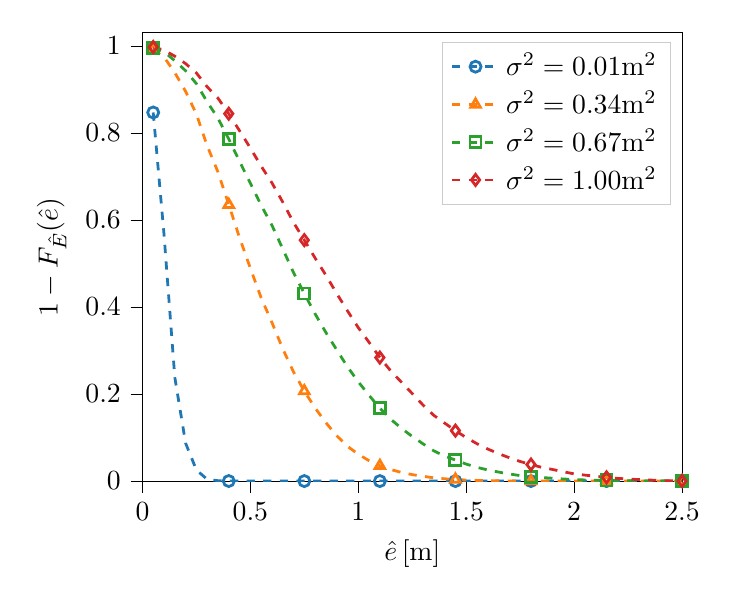
\begin{tikzpicture}

\definecolor{color0}{rgb}{0.12156862745098,0.466666666666667,0.705882352941177}
\definecolor{color1}{rgb}{1,0.498039215686275,0.0549019607843137}
\definecolor{color2}{rgb}{0.172549019607843,0.627450980392157,0.172549019607843}
\definecolor{color3}{rgb}{0.83921568627451,0.152941176470588,0.156862745098039}

\begin{axis}[
% width=1\linewidth,
legend cell align={left},
legend style={fill opacity=0.8, draw opacity=1, text opacity=1, draw=white!80!black},
tick align=outside,
tick pos=left,
x grid style={white!69.0196078431373!black},
xlabel={$\hat{e} \left[ \si{m} \right]$},
xmin=0, xmax=2.5,
xtick style={color=black},
y grid style={white!69.0196078431373!black},
ylabel={$1 - F_{\msf{\hat{E}}}(\hat{e})$},
ymin=0, ymax=1.03,
ytick style={color=black}
]
\addplot [dashed, semithick, color0, line width=1, mark=o, , mark options={solid, color0}, mark repeat=7]
table {%
0.05 0.84684
0.1 0.567
0.15 0.23832
0.2 0.0872200000000001
0.25 0.0254400000000001
0.3 0.00404000000000015
0.35 0.000880000000000103
0.4 0.0001000000000001
0.45 1.11022302462516e-16
0.5 1.11022302462516e-16
0.55 1.11022302462516e-16
0.6 1.11022302462516e-16
0.65 1.11022302462516e-16
0.7 1.11022302462516e-16
0.75 1.11022302462516e-16
0.8 1.11022302462516e-16
0.85 1.11022302462516e-16
0.9 1.11022302462516e-16
0.95 1.11022302462516e-16
1 1.11022302462516e-16
1.05 1.11022302462516e-16
1.1 1.11022302462516e-16
1.15 1.11022302462516e-16
1.2 1.11022302462516e-16
1.25 1.11022302462516e-16
1.3 1.11022302462516e-16
1.35 1.11022302462516e-16
1.4 1.11022302462516e-16
1.45 1.11022302462516e-16
1.5 1.11022302462516e-16
1.55 1.11022302462516e-16
1.6 1.11022302462516e-16
1.65 1.11022302462516e-16
1.7 1.11022302462516e-16
1.75 1.11022302462516e-16
1.8 1.11022302462516e-16
1.85 1.11022302462516e-16
1.9 1.11022302462516e-16
1.95 1.11022302462516e-16
2 1.11022302462516e-16
2.05 1.11022302462516e-16
2.1 1.11022302462516e-16
2.15 1.11022302462516e-16
2.2 1.11022302462516e-16
2.25 1.11022302462516e-16
2.3 1.11022302462516e-16
2.35 1.11022302462516e-16
2.4 1.11022302462516e-16
2.45 1.11022302462516e-16
2.5 1.11022302462516e-16
};
\addlegendentry{$\sigma^2 = 0.01\si{m^2}$}
\addplot [dashed, semithick, color1, line width=1, mark=triangle, mark options={solid, color1}, mark repeat=7]
table {%
0.05 0.99164
0.1 0.97418
0.15 0.93836
0.2 0.89532
0.25 0.8431
0.3 0.77028
0.35 0.7101
0.4 0.63504
0.45 0.55912
0.5 0.48902
0.55 0.4211
0.6 0.36426
0.65 0.30404
0.7 0.25072
0.75 0.20682
0.8 0.168
0.85 0.1342
0.9 0.10428
0.95 0.0799
1 0.06162
1.05 0.04676
1.1 0.03518
1.15 0.02646
1.2 0.01992
1.25 0.0148400000000001
1.3 0.0109800000000001
1.35 0.00744000000000011
1.4 0.00528000000000006
1.45 0.00370000000000004
1.5 0.00240000000000007
1.55 0.00156000000000012
1.6 0.000980000000000092
1.65 0.000640000000000085
1.7 0.000400000000000067
1.75 0.000280000000000058
1.8 0.000140000000000029
1.85 8.000000000008e-05
1.9 4.000000000004e-05
1.95 2.000000000002e-05
2 2.000000000002e-05
2.05 2.000000000002e-05
2.1 0
2.15 0
2.2 0
2.25 0
2.3 0
2.35 0
2.4 0
2.45 0
2.5 0
};
\addlegendentry{$\sigma^2 = 0.34 \si{m^2}$}
\addplot [dashed, semithick, color2, line width=1, mark=square, mark options={solid, color2}, mark repeat=7]
table {%
0.05 0.995659305488878
0.1 0.986297807649224
0.15 0.965834533525364
0.2 0.942650824131861
0.25 0.913106096975516
0.3 0.871219395103217
0.35 0.83359337493999
0.4 0.785765722515603
0.45 0.7344375100016
0.5 0.684249479916787
0.55 0.633661385821731
0.6 0.587734037445991
0.65 0.533645383261322
0.7 0.478896623459754
0.75 0.430768923027684
0.8 0.384161465834534
0.85 0.341294607137142
0.9 0.301548247719635
0.95 0.262481997119539
1 0.228196511441831
1.05 0.196971515442471
1.1 0.16736677868459
1.15 0.142222755640903
1.2 0.121219395103217
1.25 0.102476396223396
1.3 0.0856337013922228
1.35 0.0694511121779485
1.4 0.0575492078732598
1.45 0.0483077292366779
1.5 0.0389862377980478
1.55 0.0315450472075532
1.6 0.0255240838534165
1.65 0.0207233157305169
1.7 0.0163026084173468
1.75 0.0125620099215874
1.8 0.0100816130580892
1.85 0.00820131220995346
1.9 0.0065010401664265
1.95 0.00480076812289953
2 0.00348055688910209
2.05 0.00260041606657047
2.1 0.0019203072491597
2.15 0.00152024323891808
2.2 0.00110017602816437
2.25 0.000840134421507321
2.3 0.000500080012801885
2.35 0.000240038406144838
2.4 0.000180028804608545
2.45 8.00128020481683e-05
2.5 -2.22044604925031e-16
};
\addlegendentry{$\sigma^2 = 0.67 \si{m^2}$}
\addplot [dashed, semithick, color3, line width=1, mark=diamond, mark options={solid, color3}, mark repeat=7]
table {%
0.05 0.99719264472919
0.1 0.990214361627464
0.15 0.976077322585173
0.2 0.959112875734424
0.25 0.937576450299785
0.3 0.905813230664341
0.35 0.879744931721109
0.4 0.843971204555937
0.45 0.804788545990495
0.5 0.765144679059135
0.55 0.723615873588803
0.6 0.685115001303415
0.65 0.641019471014057
0.7 0.594096532916241
0.75 0.553590406865989
0.8 0.512402494535684
0.85 0.472999258056107
0.9 0.43094908660691
0.95 0.391084641761415
1 0.352483506787784
1.05 0.31879524353807
1.1 0.283763460265897
1.15 0.253303655577613
1.2 0.227155146483787
1.25 0.201126952615853
1.3 0.174657602919649
1.35 0.150975555956606
1.4 0.133188955062263
1.45 0.115903667609136
1.5 0.0998415849525757
1.55 0.0858248611361767
1.6 0.0736128657081553
1.65 0.0630251258296737
1.7 0.0535603280595158
1.75 0.0450781046341413
1.8 0.0379995588441716
1.85 0.0315025366460124
1.9 0.0266498225350417
1.95 0.0214361627463954
2 0.0165433435601273
2.05 0.0136958832140205
2.1 0.0110489482444001
2.15 0.00858248611361745
2.2 0.00633660189696983
2.25 0.00465218873448414
2.3 0.00338887886261985
2.35 0.00240630451783652
2.4 0.00134352002245863
2.45 0.00052136597886443
2.5 -2.22044604925031e-16
};
\addlegendentry{$\sigma^2 = 1.00 \si{m^2}$}
\end{axis}

\end{tikzpicture}

\end{document}